\section{THREAD}

THREAD is a low-power, low-latency wireless mesh networking protocol designed for secure and reliable IoT communication. 
It is based on open and proven standards, ensuring broad interoperability and long-term viability.
\begin{figure}[H]
    \centering
    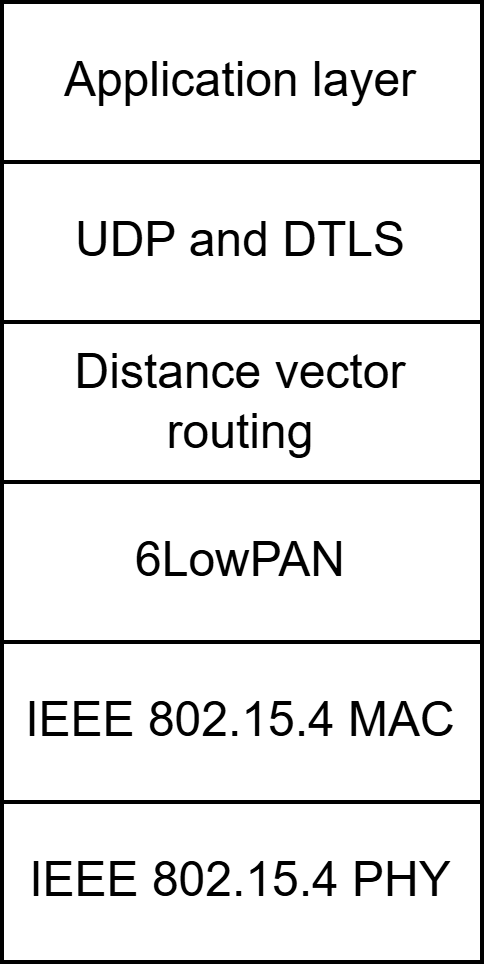
\includegraphics[width=0.25\linewidth]{images/iot15.png}
    \caption{6LowPAN protocol stack}
\end{figure}

THREAD devices are categorized based on their capabilities and roles within the mesh network:
\begin{itemize}
    \item \textit{Full THREAD Devices} (FTD): fully participate in routing and maintain a complete network topology.
        Can be divided as: 
        \begin{itemize}
            \item \textit{Router}: forward packets for other devices and provide critical services such as network joining and security.
                Routers are always powered and can dynamically downgrade to Routing-Eligible End Devices (REEDs) if necessary.
            \item \textit{Leader}: special role assigned to one router, responsible for managing the overall network structure. 
                It coordinates upgrades and other critical decisions. 
                If the leader fails, another router automatically assumes the role, ensuring network stability.
            \item \textit{Routing-Eligible End Device} (REED): a non-routing that can upgrade to a Router if the network requires it.
            \item \textit{Full End Device} (FED): does not perform routing and cannot upgrade to a router, but otherwise maintains full communication capabilities.
        \end{itemize}
    \item \textit{Minimal THREAD Devices} (MTD): a basic non-sleepy device that communicates through a parent router but does not perform routing.
        Can be divided as: 
        \begin{itemize}
            \item \textit{Sleepy End Device} (SED): a battery-powered device that conserves energy by sleeping for extended periods and only periodically waking up to communicate.
            \item \textit{Synchronized Sleepy End Device:} (SSED): a variant of the SED that synchronizes its sleep cycles for more predictable communication patterns.
            \item \textit{Bluetooth End Device}: a device that supports Bluetooth Low Energy (BLE) alongside THREAD to enable flexible connectivity options.
        \end{itemize}
    \item \textit{Border router}: connects the THREAD network to external networks, allowing seamless communication between THREAD devices and the broader Internet. 
\end{itemize}

\begin{figure}[H]
    \centering
    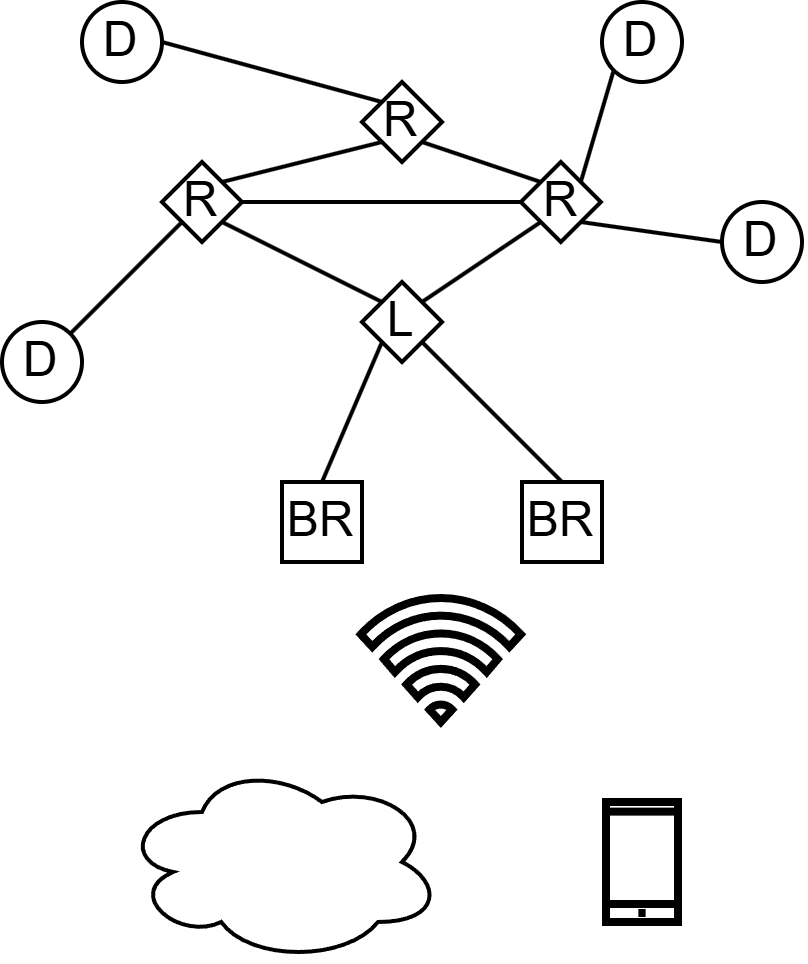
\includegraphics[width=0.35\linewidth]{images/iot17.png}
    \caption{THREAD network structure}
\end{figure}

\subsection{IPv6 over Low-power Wireless Personal Area Networks}
6LowPAN is an adaptation layer designed to enable IPv6 communication over low-power wireless networks. 
It addresses several critical challenges inherent in these networks, such as limited frame size, energy efficiency, and the need for auto-configuration. 
By providing a framework for efficient communication, 6LowPAN bridges the gap between traditional IP-based networking and resource-constrained wireless environments.

\begin{figure}[H]
    \centering
    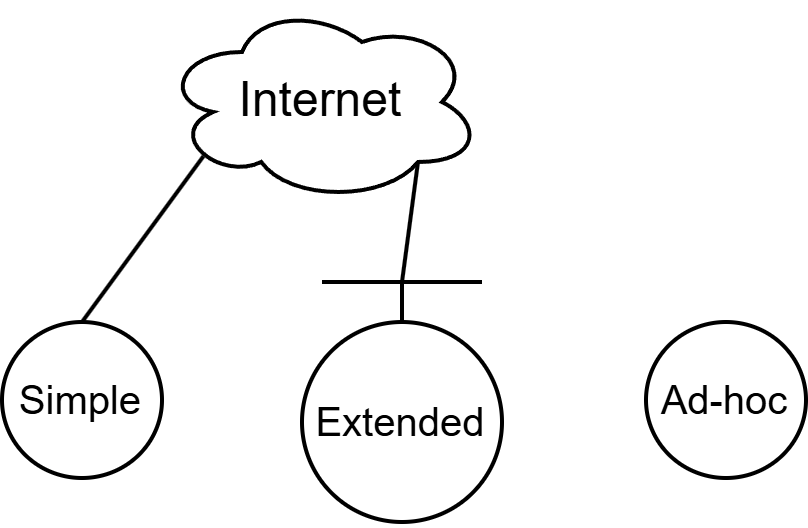
\includegraphics[width=0.5\linewidth]{images/iot18.png}
    \caption{6LowPAN architecture}
\end{figure}
The architecture of 6LowPAN involves various types of networks. 
A simple LoWPAN typically consists of a single edge router, while an extended LoWPAN incorporates multiple edge routers connected via a common backbone link. 
An Ad-hoc LoWPAN , on the other hand, operates independently without external routing. 
These networks face significant challenges when integrating with the broader Internet application protocol compatibility, IPv4 inter-connectivity, firewalls, NATs, and security concerns.

\subsubsection{Header compression}
One of the key features of 6LowPAN is its ability to perform efficient header compression.
This allows the large IPv6 headers, along with extension headers and UDP headers, to be compressed into smaller formats suitable for low-power wireless links. 
The initial specification for this was defined in RFC4944, with ongoing updates provided by draft-ietf-6LowPAN-hc. 
Additionally, 6LowPAN supports fragmentation, breaking down larger IPv6 packets into smaller chunks that fit within the constrained frame sizes of technologies like IEEE 802.15.4. 

\subsubsection{Addressing}
Addressing in 6LowPAN is optimized for low-power environments.
Nodes within a 6LowPAN network often share a common prefix, allowing for efficient compression of IPv6 addresses. 
Interface identifiers are typically derived from the link-layer address during auto-configuration, further reducing the overhead of address management. 
Network auto-configuration is achieved through neighbor discovery mechanisms, enabling seamless integration into existing infrastructures. 
Communication support includes unicast, multicast, and broadcast modes, with multicast being compressed and mapped to broadcast for efficiency.

\subsubsection{Routing}
Routing in 6LowPAN leverages protocols like IETF RPL (Routing Protocol for Low-Power and Lossy Networks), which is specifically designed for resource-constrained environments. 
RPL builds a Destination-Oriented Directed Acyclic Graph (DODAG) based on specific objective functions, which take into account metrics.
This proactive distance-vector approach ensures adaptability to different application requirements, whether they involve home automation, commercial building automation, industrial automation, or urban environments.
When it comes to routing protocols for wireless sensor networks (WSNs), the ideal solution must balance shortest-path routes, overlap avoidance, and energy efficiency. 
Distance-vector algorithms, which associate costs with links to determine the shortest path, are commonly used. Each router maintains local next-hop information, ensuring efficient packet forwarding.
Alternatively, link-state algorithms require each node to acquire complete network information, typically through flooding, and calculate a shortest-path tree to each destination. 
Proactive routing acquires information before it is needed, while reactive routing discovers paths dynamically as required.

In the context of low-power and lossy networks, the IETF's ROLL working group has developed RPL, a proactive distance-vector routing protocol tailored for embedded applications. 
RPL supports unicast, anycast, and multicast communication, adapting to various metrics such as reliability, latency, and throughput. 
It also incorporates constraint-based routing, allowing parallel paths to be established based on specific criteria. 
Scalability is a key consideration, as RPL must accommodate diverse application requirements, from time-sensitive alarm systems to energy-optimized telemetry.

\subsubsection{Summary}
The 6LowPAN format plays a crucial role in enabling IPv6 over low-power wireless links. 
It employs stateless compression techniques to reduce the size of IPv6 and UDP headers. 
Payload length is derived from the underlying link-layer header, and source and destination addresses can be elided or compressed based on the context of the transmission. 
This approach significantly reduces overhead, making it feasible to transmit IPv6 packets over constrained wireless networks.